
\maketitle

\tableofcontents
\listoftheorems[ignoreall,show={definition,corollary,lemma,theorem}]

\section{Introduction}


Deleting content from Swarm is meant to impose a cost on retrieval of deleted content that is no less than the cost of having the entirety of the information stored from deleting to attempted retrieval. Clearly, the imposed cost cannot be greater than  this, because by storing the information (either in Swarm or on one's own drive or someplace else) always allows one to access it. Note that for those who did not access the information before it was deleted this cost is usually prohibitive.


\subsection{Access control vs. censorship}

Deleting content or revoking access to content are difficult notions. On the one hand, the digitisation and increasing ubiquity of personal data in the cloud touch on sensitivities more than ever before. On the other hand, cheap storage makes it virtually impossible to make material once seen become unseen.
In response to the former, regulators often formulate requirements on removability that fails to recognise the latter. The regulatory appeal of centralised gate-keeping is clear: in case of violation, the gate-keeper provides a  well-defined responsible party. Be it on the level of publishing platform or hosting infrastructure, the  operating entity is in control of the technology serving the content and thus lends itself as the target of legal enforcement when it comes to denying access. Such a clear course of action gives the unwary a phony sense of security when it comes to digital publishing while the real issue is swept under the rug: publishing platforms have the technological means to filter content. However, such centralised control always provides an attack surface, since it makes exerting influence on content cheaper.  What starts out as sensible measures of content curation with time becomes extant censorship. This is all the more problematic with social platforms that gained quasi-monopolistic status due to network effects. As a result of high switching cost, innocent content creators sometimes end up being 'deplatformed'. Similarly, the ability to identify hosts and deny access to content via legal decree gives powers to be the means to infringe on freedom of speech. 

In the decentralised paradigm of web 3, there is no longer an operating entity behind either the publishing platform or the hosting infrastructure. Therefore, the cost of censorship is raised beyond the realm of feasibility. However, a novel approach is imminent to replace the sense of security gate-keepers purportedly represent. We argue that technology that allows sovereign control over one's own data is needed.  

\subsection{Deletion and revoking access}

First, notice that any reference to removal of information in the sense of erasing it from all physical storage devices is both unenforceable and impractical. Even the strictest data protection audits do not require the erasure of offending data from backup tapes. In general, the tacit assumption is that information ordered to be removed become inaccessible through \emph{typical precedented methods of access}.

In this paper, we aspire to formulate the strongest meaningful definition of deletion applicable to decentralised storage and offer a construction that implements it.
Importantly, such a construction needs to be purely technical, referring to primary actors' capabilities and costs as opposed to procedural, referring to intermediaries' obligations to respect the rights of primary actors. 

Primary actors here are the \emph{uploader} that wishes to share content by granting read access to a number of parties, called \emph{downloaders}. Deletion is simply reformulated as revoking access
to the content from all parties including oneself. Granting access is defined as providing some canonical \emph{reference} to the content that the system can eventually resolve to the full information meant to be disclosed. Any party that is privileged to access this information, is able to store, re-code and potentially disseminate the content seen at any later point in time including whatever process would qualify as deleting or removing access. There is, by definition, no protection possible against such adversity, hence retrospective revocation of access (and therefore deletion) is meant to be used in a narrower sense. Practically, the notion of revoked access needs to be defined in terms of \emph{the viability to replay the same access method} or any action that would allow the adversary to access information after their access is revoked for a cost lower than the cost of storing information totaling the entire size of the content shared for the entire period starting at the time the content is shared.

The scheme for content with access revocation has the following requirements: 

\begin{itemize}
    \item \emph{specialisation} - Uploader is able to choose at the time of publishing a specialised construct allowing retrospective revocation of access.
    \item \emph{sovereignity} -- Uploader is the sovereign owner of the data and is in sole possession of the means to selectively revoke access from any party previously granted access.
    \item \emph{security} -- After revocation of access, grantee is unable to access the content with the reference granting access, or any other cue that incurs less cost than the cost of storing the information in its entirety.
\end{itemize}


From a user's perspective, content that is meant to be reliably deleted should be uploaded as such. The costs of uploading such content is allowed to be a (small integer) multiple of the cost of regular, censorship-resistant uploads. 

The uploader's credentials are necessary to delete their own deletable content. Deletables must also allow access control, i.e., only available to a specific set of recipients.

The point of deleting is that if the downloader has NOT stored at least as much information as the deleted information itself, they will have no way of retrieving it. In particular, retaining the reference used to download the content in the first place will no longer be sufficient after it has been deleted. However a stronger statement is that no other information shorter than the deleted content will suffice.


\subsection{Immutable storage and access through references}

Swarm's core layer is a peer to peer overlay network that implements a distributed storage model called \emph{DISC (distributed immutable store of chunks)}, see figure \ref{fig:disc}).  Some information is said to be available in Swarm if one can retrieve it using a \emph{reference} that is (much) shorter than the information itself and is in fact constant in the length. 


\begin{figure}[htbp]
  \centering
    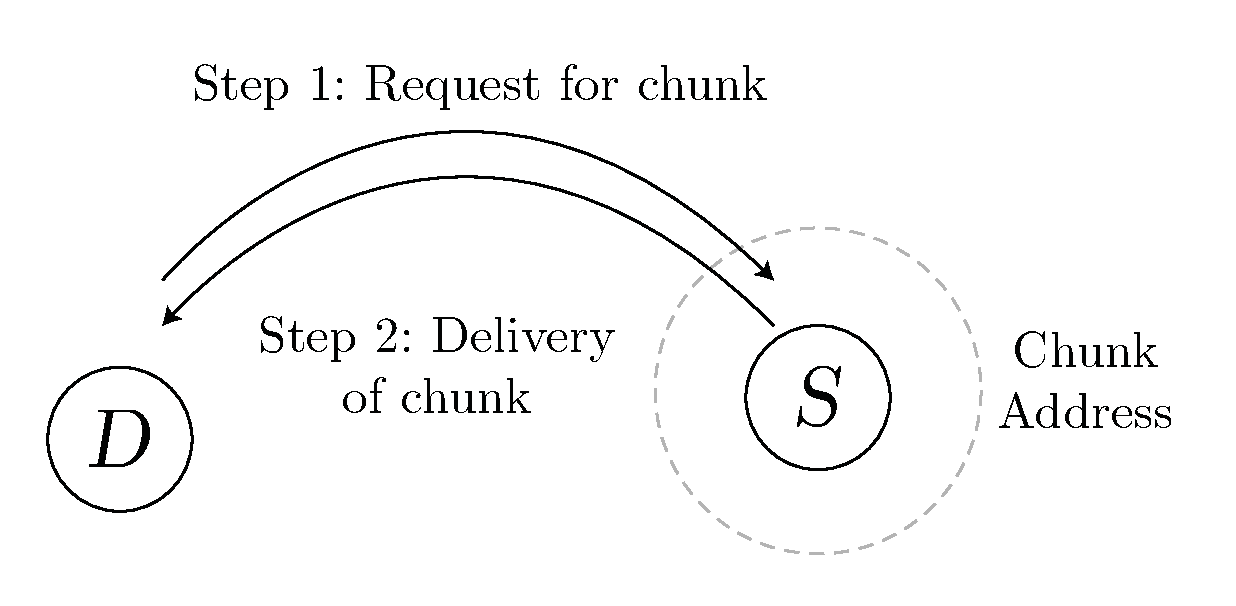
\includegraphics[width=0.8\textwidth]{figs/disc.pdf}
  \caption{DISC}
\label{fig:disc}
\end{figure}

For example, a \emph{Swarm hash}, or a Swarm hash with a \emph{decryption key}  or a \lstinline{bzz:} link.  These references are collision-free content addresses and therefore are immutable.%
%
\footnote{Even is we use mutable references, e.g., an ENS address, or feed (based on single owner chunks), these can be resolved at the time to a content address.  Whoever obtains this information can store the resolved primary reference which can later be accessed as long as assumptions about data retention in the blockchain and/or Swarm hold.} 
%
Swarm is a decentralized network where individual participants cannot (and should not) be trusted to play by the rules; it is the built-in incentives that encourage cooperative behavior and help maintain it, it being a Nash-equilibrium. The condition for content deletion to be achieved is that in \emph{at least one neighborhood} all nodes are honest, i.e., do not operate a malicious node which would store and serve information that they should not store and serve. With the growth of the Swarm network, the number of neighborhoods increases whereas the membership of neighborhoods remains about the same. Thus, the costs of attacking the proposed scheme are expected to go up.

One cooperative neighborhood suffices, that is. Of course, a powerful adversary can infiltrate every neighborhood of Swarm and archive all information that has ever been uploaded (without being able to decipher it!) and keep logs of what has been uploaded in what order, which would allow it to serve up deleted content on demand. But there is a huge price on such indiscriminate archiving of all Swarm's content and that is the only way reliably defeat the cryptographic construction that we propose for deleting.
                                   

Note that normally uploaded content may be \emph{forgotten}: if nobody pays for storing it and it is not accessed sufficiently often, the chunks constituting it will be garbage collected. However, these cannot be reliably deleted in the above defined sense. 

\section{Construction}

The goal of this section is to arrive at a formal construction of a DISC-based revocable access model. We will restrict our scheme to \emph{chunks}, the fundamental fix sized storage unit of Swarm's DISC model.  The proposed \emph{dream} construct implements a  deletable content storage and access model conforming to the requirements of specialisation, sovereignty, and security. The use of the word 'dream' alludes to the somewhat unexpected finding that such a construct is even possible in the immutable DISC model. On top of this, as customary in swarm, it serves as a mnemonic acronym, resolving to the 5 \emph{dream attributes} of access control.

\begin{itemize}
    \item[\textbf{d}] \emph{deniable} -- the dream key serves as a one time pad for decryption. Since multiple content chunks (in fact any arbitrary content) can use the same dream pad, the key's association to any content is plausibly deniable.
    \item[\textbf{r}] \emph{revocable} -- access granted by dream keys is revocable. Revoking access from all parties including oneself is taken as deletion.   
    \item[\textbf{e}] \emph{expirable} -- the scheme allows for one-time use, i.e., the key can only be retrieved once
    \item[\textbf{a}] \emph{addressable} -- access can be granted to a neighbourhood, only clients operating a node with an overlay address in a given range  are able to access
    \item[\textbf{m}] \emph{malleable}  --  the construct is resilient to churn and dynamic change of network size, is reusable across independent grantees and upgradeable.

\end{itemize}

The scheme is built on top of DISC's APIs and can be implemented entirely as a second layer solution.  Despite the rich feature set, the scheme is not a complex cryptographic scheme, rather relies on the interplay of various levels and component subsystems.

\begin{itemize}
    \item \emph{one time pad} -- Dream content is reconstructed by xor-ing two equal-length parts. This scheme is shared by a construct designed  for plausibly deniable content.
    \item \emph{authorised mutability} -- finding a scheme where retrieval will rely on an interactive protocol.
    \item \emph{incentives} -- the smooth operation of the interactive protocol is guaranteed by the systemic incentives, however, correctness should not depend on them. Abuse of the intention, should be prohibitively costly to incentivise. 
\end{itemize} 







\subsection{Prerequisites}

\subsubsection{Chunk upload in swarm}

When content is uploaded to swarm, the local client splits the data into 4-kilobyte chunks and pushes each chunk to the network using the \emph{pushsync} protocol. This protocol is responsible for transmitting a chunk newly entered to the neighbourhood where it will be retrieved, i.e., the neighbourhood closest to the content address of the chunk. See figure \ref{fig:pushsync}. 

\begin{figure}[htbp]
  \centering
    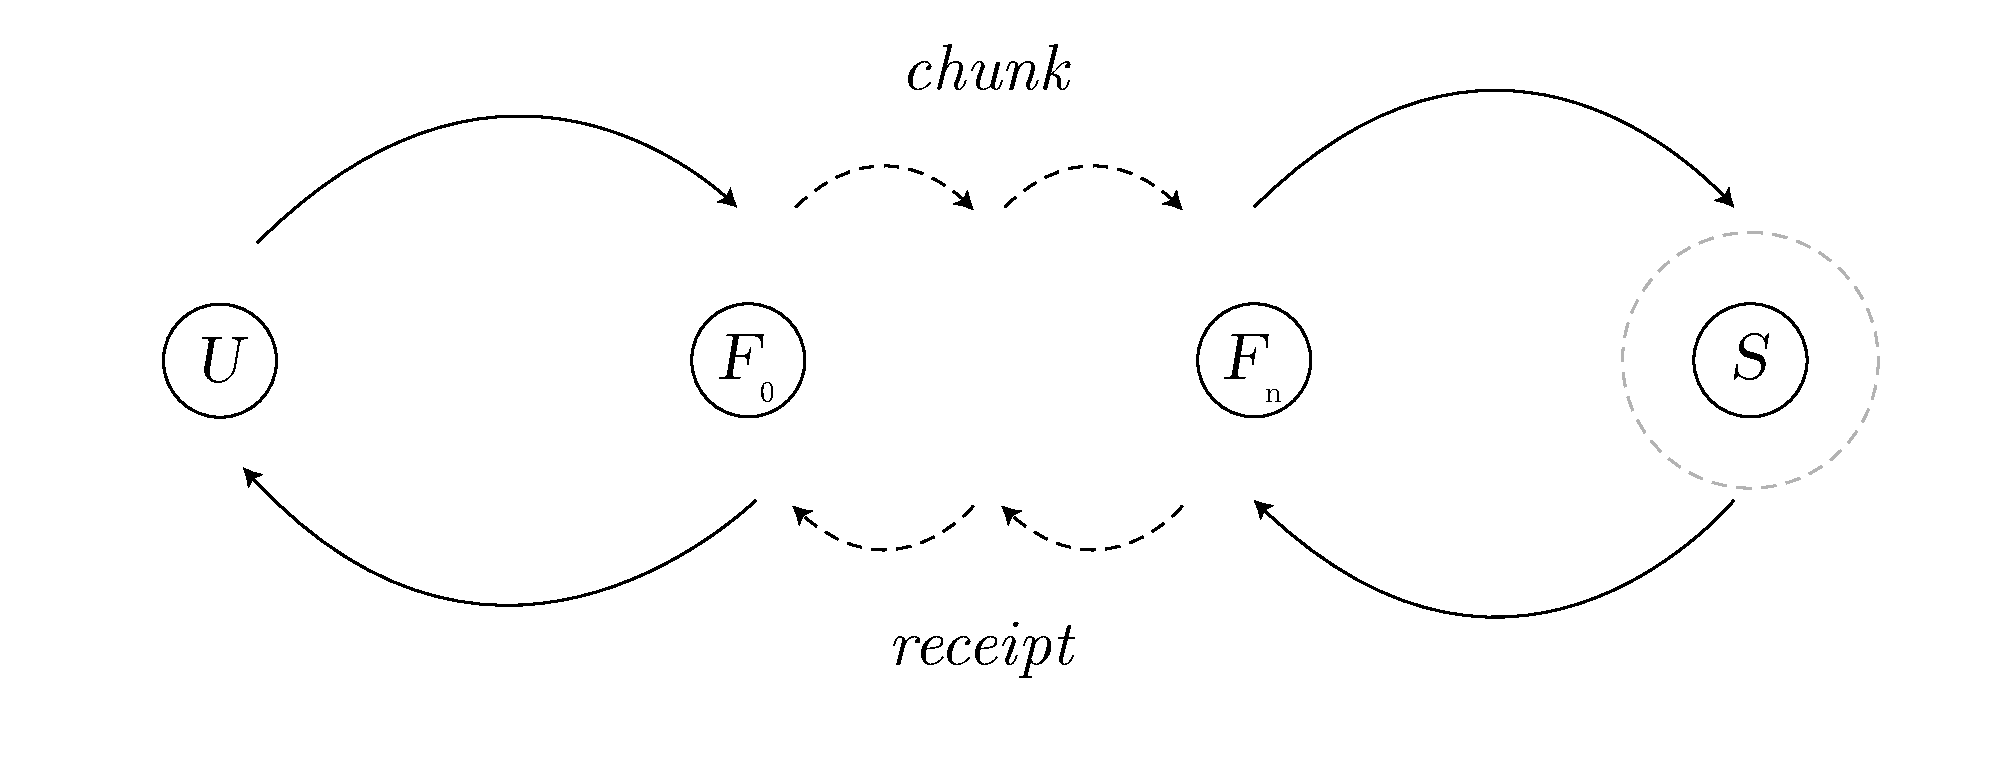
\includegraphics[width=0.8\textwidth]{figs/push-sync.pdf}
  \caption{Push syncing.}
\label{fig:pushsync}
\end{figure}



Network protocol in swarm use forwarding Kademlia routing meaning that queries reach their target neighbourhood by being relayed through a series of hops by nodes with ever increasing proximity to the target address.

The chunk delivery to storer nodes can also be seen as a request: the closest node respond with a statement of custody that is passed back via the same route as the original request (\emph{backwarding}). 
When uploading content, a measure must be present that would prevent mass injection of random chunks to the network. By requiring \emph{postage stamps}, we impose an upfront cost to uploads which is an effective measure against spamming, i.e., makes it costly to flood the network with chunks and as a consequence expunge valuable chunks from the network by triggering garbage collection on nodes with  capacity shortage. The attached postage stamp can serve as a signal to the  importance of keeping a chunk.

As an extention to this idea, the central postage stamp contract operates a system of redistribution called \emph{postage lottery}  whereby the pool of funds cumulating from all postage revenue is reallocated to unstaked storer nodes in return for proof of custody on chunks with valid stamps.

This system is responsible for positive storage incentives. More relavant to push syncing, the promise of storage revenue from the postage lottery race bestows a value on a chunk with a postage stamp and renders the pushsynced chunks a valueable commodity for the nodes close to them.
An intermediate node is incentivised to forward a chunk towards its address because the node it passes the chunk on to will pay more for it than what the node buys it for. As an important corollary to this, a node will always have the incentive to push a chunk if they do not need to pay for it or if they can make sure they are compensated.

\begin{lemma}[uploaded chunks travel to neighbourhood]
\label{lem:pushsync}
Every chunk uploaded to swarm is pushsynced and is forwarded by each relaying node towards its address  provided it has a valid postage stamp attached. As a consequence of Kademlia connectivity, the route to the node whose address is closest to the chunk can be found using local decisions by the nodes intermediate in the path. As a result of incentivised push syncing, a chunk with a valid postage stamp will end up being received by at least the closest node. Due to synchronisation of chunks among the nodes in a neighbourhood, the chunk will end up being received by each node in the neighbourhood of its address.
\end{lemma}

\subsubsection{Single owner chunks}

The DISC storage model supports two chunk types, a content addressed chunk and  single owner chunk. Content addressed chunks attain their integrity by the fact that their address is deterministically derived from their content with the help of a one-way uniform digest function (in particular, the binary  merkle tree hash). A single owner chunk on the other hand, encodes the association of an index and a payload sanctioned by the signature of an owner. The owner's ethereum address hashed with the index determines the chunk address. See figure \ref{fig:soc}. 

\begin{figure}[htbp]
  \centering
    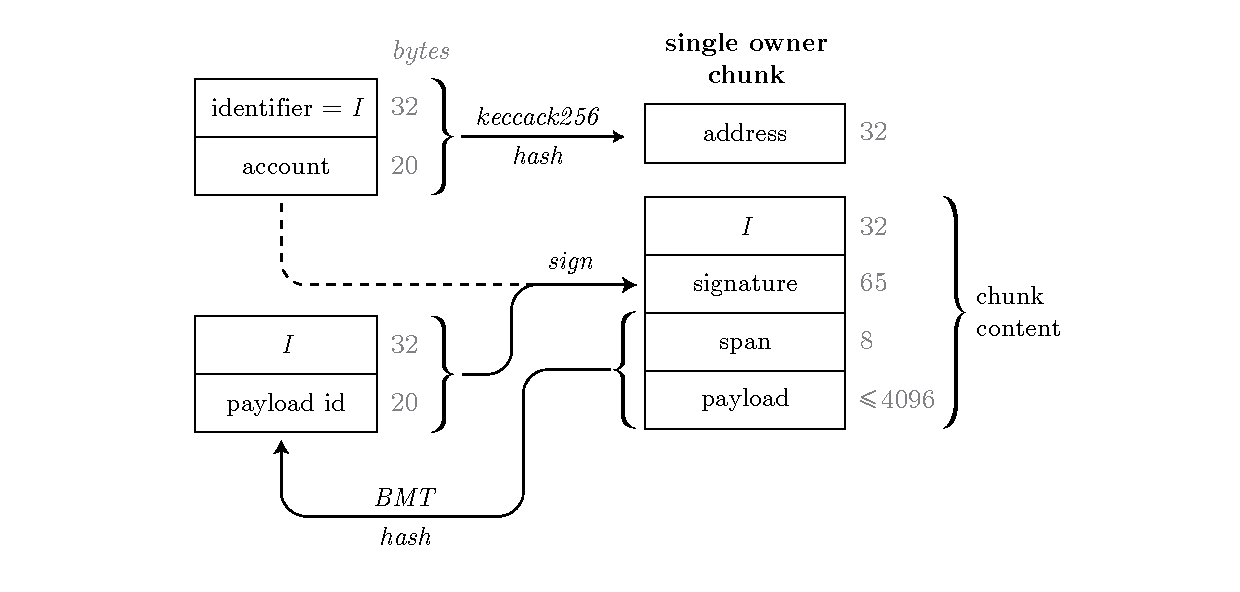
\includegraphics[width=0.8\textwidth]{figs/single-owner-chunk.pdf}
  \caption{Single owner chunks}
\label{fig:soc}
\end{figure}

Single owner chunks can wrap full length  content addressed chunks.

The hash function used to generate the content address of chunks in swarm is based on a \emph{binary merkle tree}. For ease of notation though, we just use $\mathit{H}$ to indicate a hash function. This is also appropriate since the particular choice of hash function does not affect the correctness   of our construction.  


\subsubsection{Pseudo-random sequence from generator}
Assume we have a pseudo-random deterministic function that generates a longer (e.g., chunk-sized = 4K) sequence $c$ from a key-sized (32 byte) generator $g$. For example, the Keccak sponge function used throughout Ethereum for hashing does have this capability. It is used in Swarm in order not to introduce  security assumptions in addition to those of Ethereum.

\begin{definition}[Pseudo-random sequence generation]
\label{def:gen4k}
\begin{equation}
\mathit{Gen4K}: [32]byte \mapsto [4096]byte
\end{equation}

\begin{equation}
\mathit{Gen4K}(g) \defeq \langle c_0, c_1, \ldots c_{127}\rangle
\end{equation}
with 

\begin{equation}
c_i \defeq \mathit{H}(g|i)
\end{equation}
\end{definition}


\subsection{Dream: deniable, revocable, expirable, addressable, malleable}

In what follows, through a number of steps, we introduce the \emph{dream}, a chunk-sized one time pad construction that provides the necessary mutability for content with revocable access.

Let $B$ be a set  of postage batches, owned by $U$. Without losing generality, we assume that this set is represented by a postage payment ID $b$, a 32-byte hash. 

Let \emph{Chunks(b)} denote all chunks stamped by $b$.

\begin{definition}[Nearest Chunk]
\label{def:cin}
Define  $\mathit{NC}(b,p)$ as the chunk stamped by batch $b$ with minimal XOR distance to pivot $p$.

\begin{equation}
\mathit{NC}: \mathit{Batches}\times \mathit{Chunks} \mapsto \mathit{Chunks}
\end{equation}
\begin{equation}
\mathit{NC}(b,p)\defeq \underset{c\in \mathit{Chunks}(b)}{\operatorname{arg\,min}}\chi(\mathit{H}(p),\mathit{H}(c))
\end{equation}
\end{definition}

Let us define the \emph{chunk filter} as a function that transforms an input one time pad into another output one time pad using an additional chunk.

\begin{definition}[Chunk filter function]
\label{def:chunk-filter}
\begin{equation}
f: \mathit{chunks}\times\mathit{chunks}\mapsto \mathit{chunks}
\end{equation}
such that $f$(p,C) is calculated as follows:  
\begin{equation}
    f(p,C) \defeq \mathit{Gen4K}(\mathit{H}(p|C)) 
\end{equation}
...
\end{definition}

\begin{corollary}[Chunk filter is a random oracle]
\label{cor:chunk-filter-oracle}
Follows directly from the random oracle assumption about the hash function.
\end{corollary}

Let us define the \emph{task function $T$} for the dream construct. The task function defines an one time pad transform function using the chunk filter function on a set of chunks stamped with $b$ and found in the neighbourhood of the input $p$.

\begin{definition}[Task function]
\label{def:task}
Given a batch $b$, the task function takes the nearest chunk stamped by $b$ in the  neighbourhood of the input $p$.
\begin{equation}
T: \mathit{Batches} \mapsto (\mathit{Chunks} \mapsto \mathit{Chunks})
\end{equation}
such that
\begin{equation}
\mathit{T}(b)(p)\defeq f(p,\mathit{NC}(b,p)) 
\end{equation}

\end{definition}


\begin{corollary}[Task function is a random oracle]
\label{cor:task-function-oracle}
Due to \ref{cor:chunk-filter-oracle} and the choice of input $p$, the task function serves as an effective pseudo random generator function.
\end{corollary}


\begin{corollary}[Task function local computability]
\label{cor:task-function-locality}
The task function can be calculated by storer nodes in the neighbourhood of the input. This is a consequence of the DISC storage model, specifically that nodes store chunks in the proximity of their overlay node address.

In particular, if a storer node with overlay address $a$ stores all chunks $c_i$ where $\mathit{PO}(a,\mathit{H}(c_i))\geq d$ for some depth $d$ and $\mathit{PO}(a,\mathit{H}(p))\geq d$ as well for pivot $p$ then if it stores at least one chunk from batch $b$, it also stores $NC(b,p)$, because it implies that $a$, $\mathit{H}(p)$ and $\mathit{H}(NC(b,p))$ have a common prefix of length $d$.

If, however, $\mathit{PO}(a,\mathit{H}(NC(b,p)))<d$ then the computation of the task function fails, as the node does not store any chunks from $b$.

As long as all storer nodes store at least one chunk from $b$ and the entire address space is covered with storer nodes, the task function is computable by the storer node with overlay address $\underset{a\in S}{\operatorname{arg\,min}}\chi(\mathit{H}(p), a)$ where $S$ is the set of all storer nodes.
In particular the $\mathit{PO}(p,\mathit{NC}(b,p))$ should always be greater than the storer nodes neighbourhood depth. Conversely, if swarm grows and the density of storer nodes is so high that there is a node whose neighbourhood  depth is higher than the the minimum PO used for nearest chunks, then computability of the task function cannot be guaranteed. 

This practically means that the dream imposes a minimum density requirement on batches. Let us use the term network depth for this minumum value.

%This reduces to proving that such a node has all the chunks in $\mathit{CiN}(b,d,h)$. 
%If the value  of chunk in  $b$ is   higher than the cut off value, then the node should not have deleted any chunk in $\mathit{chunks}(b)$.% 
% 
%\footnote{This translates to the requirement that batch  $b$ has sufficient chunk balance as witnessed on the blockchain.}   
%
%As long as it  had received all chunks it will have all chunks within its storage radius $r$, $\mathit{CiN}(b,r,o)$. We need to show that the chunks needed  to calculate the task function are a subset of this, i.e., 
%$\mathit{CiN}(b,d,h) \subseteq \mathit{CiN}(b,r,o)$. 

%Since $o$  is closest to $h$, $PO(o,h)\geq r$.
%Therefore $\mathit{CiN}(b,r,o) =  \mathit{CiN}(b,r,h)$.
%As $d>r$ by  construction, $\mathit{CiN}(b,d,h)\subseteq %\mathit{CiN}(b,r,h)$.  \qedsymbol
\end{corollary} 

Since the task function can be applied to its own output, we can define the one time pad chain function using a generic \emph{chaining} construct:

\begin{definition}[Chaining]
\label{def:chaining}
\begin{equation}
\mathit{Chain}: (X \mapsto X) \times X \mapsto (\mathbb{N} \mapsto X)
\end{equation}
such that
\begin{equation}
\mathit{Chain}(f,g)(i)\defeq\begin{cases}g&\text{ if }  i=0\\
f(\mathit{Chain}(f,g)(i-1)) & \text{otherwise}
\end{cases}
\end{equation}
\end{definition}

This allows us to define the \emph{dream chain}.

\begin{definition}[Dream chain]
\begin{equation}
\mathit{DreamChain}: \ma  thit{Batches}\times \mathit{Keys} \mapsto (\mathbb{N} \mapsto \mathit{Chunks})
\end{equation}
such that
\begin{equation}
\mathit{DreamChain}(b,g) \defeq \mathit{Chain}(T(b),\mathit{Gen4k}(g))
\end{equation}
\end{definition}


\begin{corollary}[Dream chain as pseudo-random generator]
\label{cor:dream-chain-oracle}
Due to \ref{cor:task-function-oracle}, the dream chain function is a pseudo random generator.
\end{corollary}
Now we can turn to the definition of a dream.

\begin{definition}[Deniable, revocable, expirable, addressable, malleable access method]
\label{def:dream-otp}
For step-count $n$ and authorised target address $a$ and a batch $b$ with sufficient density for network depth $d$, find the generator $g$, such that
the $n$-th one time pad output of the dream chain hashes to $a$'s neighbourhood using the same network depth $d$ that constrains nearest chunk.

\begin{equation}
\mathit{dream}(b,n,a) \subset \mathit{Keys}\times\mathit{Chunks}
\end{equation}
such that
\begin{equation}
\langle g, k\rangle \in \mathit{dream}(b,n,a) \Longleftrightarrow
k=\mathit{DreamChain}(b,g)(n)
\land
\mathit{PO}(a,H_{\mathit{bmt}}(k))\geq d
\end{equation}

\end{definition}

\begin{lemma}[Construction by batch owner]

The owner of the batch is able to construct the dream pad.

\begin{proof}
First, it is trivial to see that the owner of  $b$ has access to $\mathit{chunks(b)}$ and  therefore can  calculate $T(b)$ for any input. As a result they can also calculate $k$ given $g$. Since $\mathit{H}(k)$ is uniform, the chance of $\mathit{PO}(a,\mathit{H}(k))\geq d$ is $2^{-d}$, and thus the expected number of cycles to find the dream is $2^d$.\qed
\end{proof}
\end{lemma}


Let us  define a network protocol \emph{dream}. See figure \ref{fig:protocol}. 

\begin{figure}[htbp]
  \centering
    % \includegraphics[width=0.8\textwidth]{}
  \caption{The dream protocol}
\label{fig:protocol}
\end{figure}


\begin{definition}[Dream protocol]

Those who play the protocol, listen to single owner chunks such that $c\in\mathit{dreamable}$.
We assume that they extract the batch identifier $b$, and the payload $p$ as input to the task function and then calculate $T(b)(p)$, wrap it as a dream chunk and send it to the network.
\end{definition}

\begin{corollary}[Reception of one time pad]
\label{cor:reception}
The one time pad in the chain is received by the node closest to its address.

\begin{proof}
Follows from lemma \ref{lem:pushsync} and the wrapping construction. \qedsymbol
\end{proof}
\end{corollary}



\begin{corollary}[Continuity of the chain]
\label{cor:continuity}
Given a chain  $c=\mathit{DreamChain}(b,g)$, 
a storer node at address $o$ closest to $\mathit{H}(c(i))$ is able to calculate $c(i+1)$.

\begin{proof}
Follows from \ref{cor:task-function-locality}.
\qedsymbol
\end{proof}
\end{corollary}

In other words, the neighborhood from which to choose the chunks to calculate $T$ is within the node's area of responsibility,  and therefore the node can safely assume that it does have all the  chunks.

\begin{corollary}[Termination]
\label{cor:termination}
Given $\langle g, k\rangle \in \mathit{dream}(b,g,a)$, the chain  $c=\mathit{DreamChain}(b,g)$, 
if the protocol is followed up to $n$ steps, then $k=c(n)$ is received by the target node at address $a$. 

\begin{proof}
Follows from \ref{cor:reception} and \ref{cor:continuity}.\qedsymbol
\end{proof}
\end{corollary}

\subsection{Contructing and referencing dream chunks}

We now turn to the construction of dream chunks. 

\begin{definition}[Constructing a dream chunk]
\label{def:dream}
Uploader $U$ wishes to grant downloader $D$ (at overlay address $a$) revocable  access to content chunk $C$.
$U$  chooses a postage batch $b$ it owns that is completely filled, a step-count $n$, and a depth $d$.
$U$ creates a dream generator $\langle g, k\rangle\in\mathit{dream}(b,d,n,a)$.              

Now $U$ calculates the "ciphertext" $C'=C \xor k$ and uploads it to swarm obtaining 
$r=\mathit{H}(C')$ as reference.

Now $U$ creates the \emph{dream reference} as $\mathit{ref}(C)=\langle r,b,g\rangle $.

%This will be serialised as concatenated 97 bytes.
% $U$ gives the reference to $D$ who operates 
% a node at overlay address $a$.
\end{definition}



\begin{definition}[Retrieval]
\label{def:retrieval}
$D$ in possession of a dream chunk reference as 
$\langle r,b,g\rangle $ calculated by $U$  as $\mathit{ref}(C)$ constructs $p=\mathit{Gen4K}(g)$ and wraps it as a dream chunk and sends it to swarm. When it receives the dream chunk for $b$, it extracts payload $k$.

Then $D$ downloads $C'$ by using reference $r$, then decodes $C=C'\xor k$.
\end{definition}

\begin{lemma}[Retrieval is correct and viable]
The retrieval process described in \ref{def:retrieval} is trivially correct as long as 
\begin{enumerate}
    \item  $C'$ is retrievable through $r$. This 
    \item the dream protocol is adhered to
    \item $\mathit{NC}(b,p)$ has not changed for the neighbourhoods that are on the dream path. ($\mathit{chunks(b)}$) can only change if the owner chooses to add new chunks to the  batch which is exactly the tool to revoke access.
\end{enumerate}
\end{lemma}
is able to access $C$.


\begin{corollary}[Deniable dreams]
\label{cor:deniable}
The construction is deniable.

\begin{proof}
Beside our sensitive content $C$, take $A$, any uncontroversial content chunk. When producing $C'$, the owner also produces  $A'=A\xor k$ and upload it. When asked about $k$, producing $A$ makes the denial of other content including $C$ more plausible. \qedsymbol
\end{proof}
\end{corollary}

\begin{theorem}[Access control is correct]
\label{the:accessm}
As long as $\mathit{chunks}(b)$ is unchanged, $D$ launches a retrieval as per \ref{def:retrieval}, they will indeed receive chunk $k$ at address $a$. Once they can access content $C$.

Notice that  $D$ is unable to access $C$ at any other neighbourhood.
\begin{proof}
Follows from \ref{cor:termination}.   \qedsymbol
\end{proof}
\end{theorem}

We are now turning to access revocation. Deletion of content is equivalent to revoking all access.

\begin{definition}[revoking access to a dream chunk]
\label{def:revoking}

Uploader $U$ had granted $D$ (at address $a$) access to $C$ through the dream reference $\langle r,b,g\rangle $. $U$ revokes access from $D$ by uploading extra chunks to batch $b$ such that $\mathit{NC}$ changes.
\end{definition}

\begin{theorem}[revoking access is correct]
\label{the:revoking}

As long as there is a single honest neighbourhood walked by the protocol, such that the nearest chunk to pivot $p$ from batch $b$ changes, then $D$ can no longer retrieve $C$.

\begin{proof}
Let us assume that there is an $i$ such that $\mathit{NC}(b,H(c(i)))$ changed since uploader constructed the dream. Now, when the node in the neighbourhood of $H(c(i))$ calculates the task function, the result will be completely different (see \ref{cor:dream-chain-oracle}). \qedsymbol
\end{proof}
\end{theorem}

\section{Analysis}

\subsection{Incentives}

Discuss the reliability of the protocol in the context of economic incentives.
\begin{figure}[htbp]
  \centering
    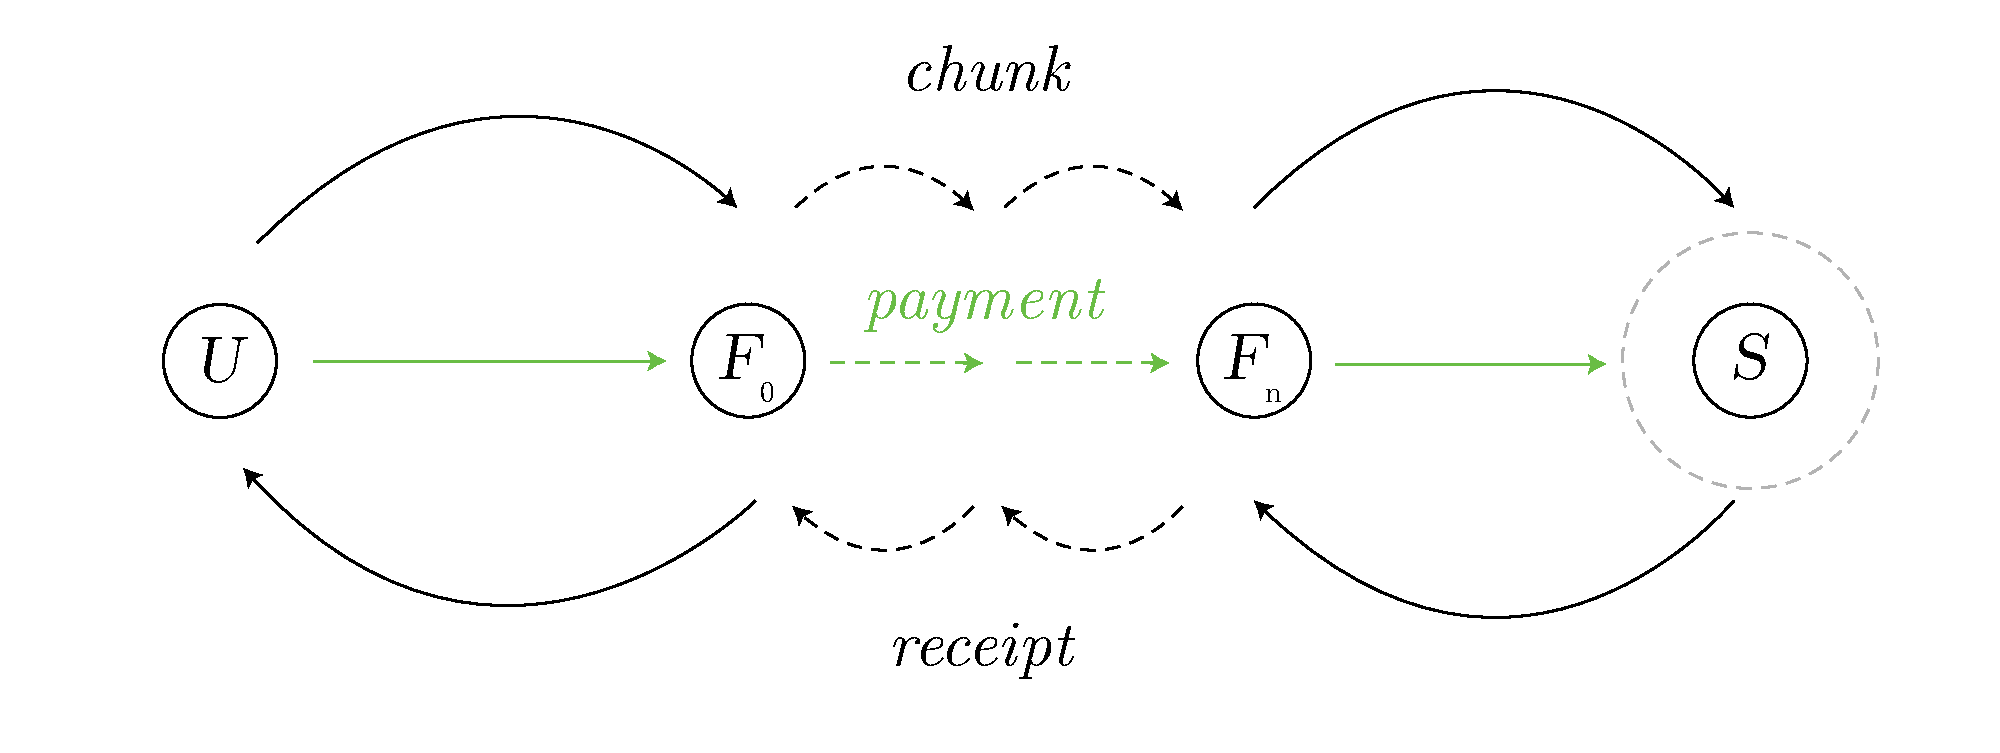
\includegraphics[width=0.8\textwidth]{figs/push-payment.pdf}
  \caption{Incentives for push syncing.}
\label{fig:push-payment}
\end{figure}



How to determine when to forward.

discuss the cost of a dream
\subsection{Security}

We now turn to the discussion how to calibrate the step-count given a security model. Let us assume a network-wide neighbourhood infiltration rate of $\frac{1}{2}$, meaning that  half of the neighbourhoods in the network is assumed  to be  malicious and colluding. 

Assuming that when  revoking access, the owner uploaded new chunks in each neighbourhood on the dream path. We assume that malicious nodes are able and willing to disregard these  new chunks and in an attempt to facilitate abuse of revoked access respond to the dream protocol just like  before the revocation.
If each  neighbourhood  on  the path comes from $M$, it is in principle possible that the dream protocol gives the unchanged response, and access is abused, i.e., allowed even though it is revoked.
However even if even  a single neighbourhood on the dream path is honest they respect the newly arrived chunks and divert the dream path, making it never terminate with the grantee. 

Thus for  a breach to happen, all neighbourhoods should come from $M$.
Which neighbourhood is malicious is not known, therefore the choice of neighbourhood in the construction is considered independent. when choosing $n$ nodes, the probability of each being malicious is $2^{-n}$. So for an infiltration of $\frac{1}{2}$, and a security requirement of $99.9\%$, $n=10$, for $99.9999\%$, $n=20$ will suffice. For an infiltration of $\frac{1}{32}$, and a security requirement of $99.9\%$, $n=2$, for $99.9999\%$, $n=4$ will suffice. 

Note that the reference does not leak either the step-count or any other information about the neighbourhoods touched. Moreover, participants in the protocol also do not know either at which position they are on the chain or anything  about the other neighbourhoods except for the following one to which they are push-syncing their chunk.

Discuss ways nodes could collude to circumvent the intention of deletion


\subsection{Dream files}

Generalise from chunks to files. 

\section{Conclusion}





% Since these parts are symmetrical, it is somewhat misleading to refer to them as ciphertext and key.  However, in the deletable construct one part will be available via a normal hash reference, this we can call one time pad, while the ephemeral part is called encoded content. 


% There is also a variation that "self-destructs", i.e. that deletes itself upon
% retrieval, but it is important to understand that it is a very fragile
% mechanism with no guarantee that the intended recipient will be able to
% download it even once. It should only be used in settings where the recipient can,
% for a limited time, request re-uploading in case the content gets deleted
% without all its parts reaching the recipient. 



% \begin{definition}[pss encode function]

% \begin{equation}
% \Psi(b,d,c)=\mathit{Trojan}(\mathit{nonce}, \mathit{topic}, \mathit{payload})
% \end{equation}
% where
% \begin{equation}
% \mathit{nonce} = c[0:32]
% \end{equation}
% \begin{equation}
% \mathit{topic} = \tau
% \end{equation}
% \begin{equation}
% \mathit{payload}[0:32] =  b
% \end{equation}
% \begin{equation}
% \mathit{payload}[32:34] = \mathit{bigendian.Uint16}(d)
% \end{equation}
% \begin{equation}
% \mathit{payload}[34:4030] = c[100:4096]
% \end{equation}
% \end{definition}
 